\documentclass[a4paper]{scrartcl}
\usepackage[ngerman]{babel}
\usepackage[utf8]{inputenc}
\usepackage{amssymb,amsmath}
\usepackage{graphicx}
\usepackage[inline]{enumitem}
\setlist{noitemsep}
\usepackage[binary-units=true]{siunitx}
\usepackage{hyperref}
\usepackage{parskip}
\usepackage[nameinlink,noabbrev,ngerman]{cleveref} % has to be after hyperref
\usepackage{nicefrac}
\usepackage{csquotes}
\usepackage{booktabs}  % for \toprule, \midrule and \bottomrule

\usepackage{minted} % needed for the inclusion of source code

\usepackage{xcolor}
\definecolor{magenta}{HTML}{FF00FF}

\setcounter{secnumdepth}{2}
\setcounter{tocdepth}{2}

\usepackage{wasysym}
\usepackage{microtype}

\begin{document}
\selectlanguage{ngerman}
\title{2014 Hauptklausur (WS 2013/14)}

\setcounter{section}{1}
%%%%%%%%%%%%%%%%%%%%%%%%%%%%%%%%%%%%%%%%%%%%%%%%%%%%%%%%%%%%%%%%%%%%%%%%%%%%%%
\section*{Aufgabe 1: Farben und Farbwahrnehmung}
\subsection*{Teilaufgabe 1a: Chromatizitätsdiagramm}
\begin{figure}[h]
    \centering
    \includegraphics*[width=0.8\linewidth, keepaspectratio]{1a.png}
    \caption{Aufgabe 1a}
    \label{fig:1a}
\end{figure}

\subsection*{Teilaufgabe 1b}
\textit{Welcher der Farbeindrücke aus Aufgabe a) lässt sich nicht durch monochromatisches
Licht erzeugen?}

Alles auf der Purple line. Also insbesondere \textcolor{magenta}{\textbf{Magenta}}.

\subsection*{Teilaufgabe 1c}
\begin{align}
    x &= \frac{X}{X + Y + Z}\\
    y &= \frac{Y}{X + Y + Z}
\end{align}

\subsection*{Teilaufgabe 1d}
$(2) < (3) < (1)$, also\\
RGB $<$ Raum aller Farben die durch 100 monochromatische Leuchtdioden darstellbar sind $<$ XYZ

\subsection*{Teilaufgabe 1e}
\begin{tabular}{cp{6cm}ccp{5cm}}\toprule
\#& Aussage  & Wahr & Falsch & Begründung \\\midrule
1 & Den Weißpunkt eines Farbraums bezeichnet man auch als Tristimulus\-wert. & $\square$ & \CheckedBox & Die RGB-Werte sind die Tristimulus-Werte. Der Weißpunkt heißt pblicherweise $D[\text{Zahl}]$, wobei die Zahl die Temperatur angibt. D65 hat eine Farbtemperatur von ca. 6504K.\\
2 & Die subjektiv empfundene Stärke von Sinneseindrücken ist proportional zum Logarithmus ihrer Intensität. & \CheckedBox &  $\square$    & ~          \\
3 & Jeder Farbeindruck für den Menschen kann mit drei Grundgrößen beschrieben werden. & \CheckedBox & $\square$ & 1. Graßmannsches Gesetz \\\bottomrule
\end{tabular}

\section*{Aufgabe 2: Whitted-Style Raytracing}
\subsection*{Teilaufgabe 2a-d}
Siehe \cref{fig:2a}.

\begin{figure}[h]
    \begin{minipage}[b]{0.45\linewidth}
        \centering
        \includegraphics*[width=\textwidth, keepaspectratio]{2a.png}
        \caption{Aufgabe 2a-d; $n_1 = 1, n_2 = 1.5$}
        \label{fig:2a}
    \end{minipage}
    \hspace{0.5cm}
    \begin{minipage}[b]{0.45\linewidth}
        \centering
        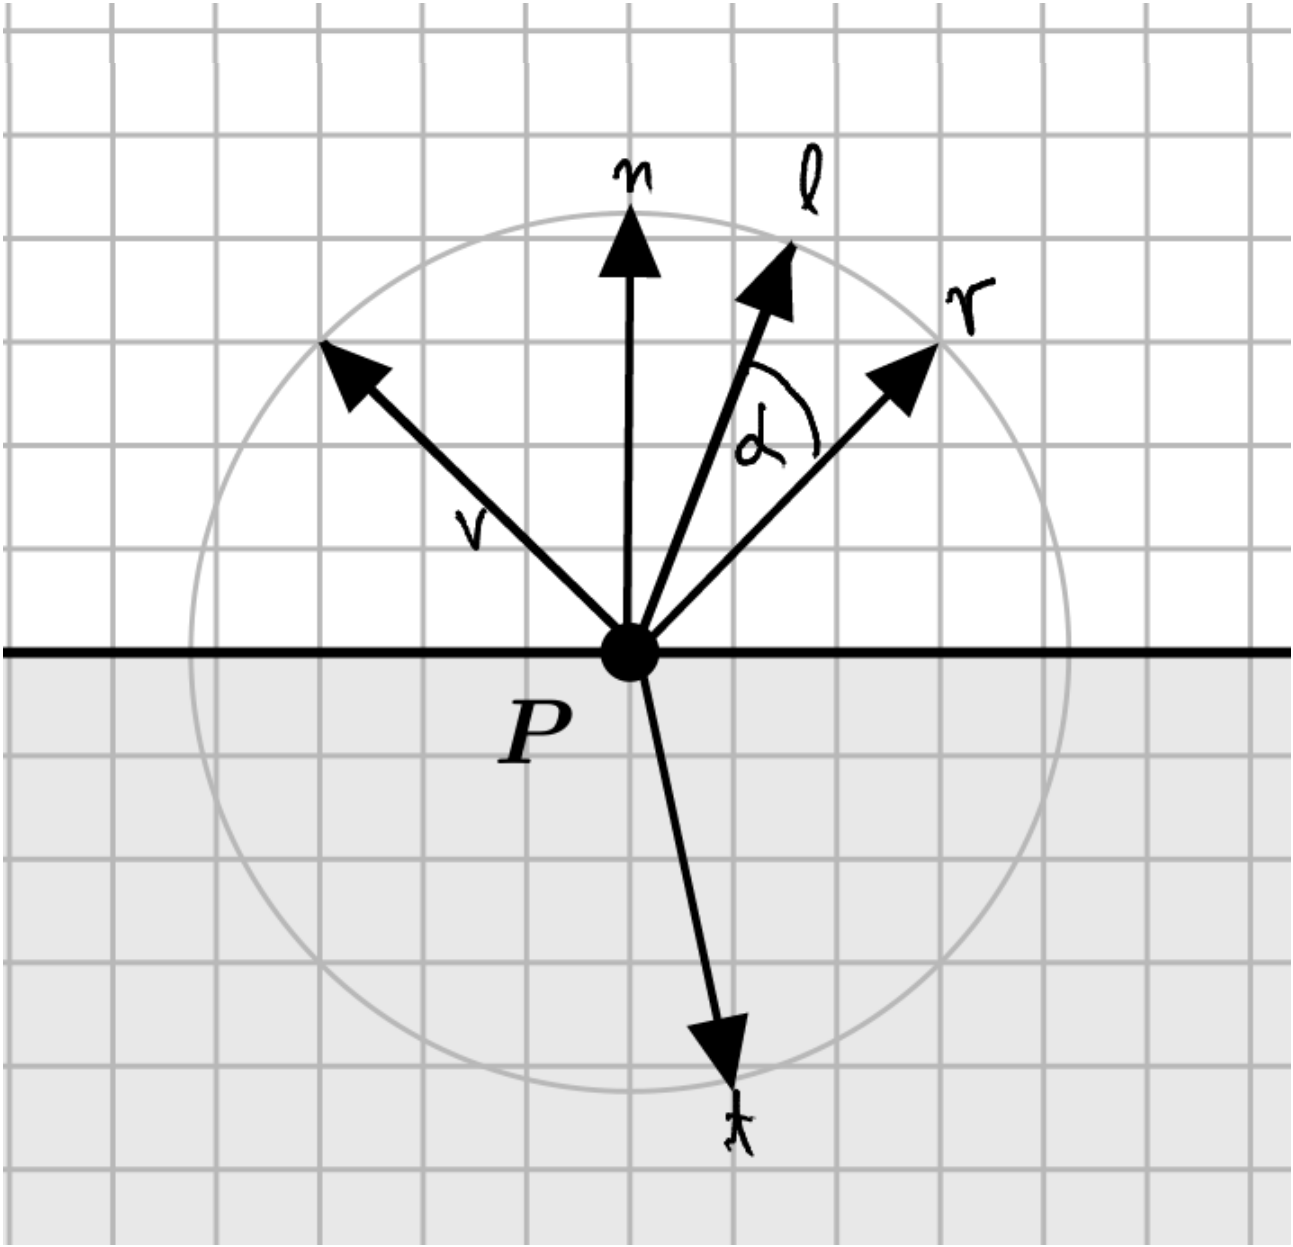
\includegraphics[width=\textwidth, keepaspectratio]{2-alternative.png}
        \caption{Alternative Lösung - kA was richtig ist. Siehe \href{https://github.com/MartinThoma/KIT-Musterloesungen/issues/10}{github.com/MartinThoma/KIT-Musterloesungen/issues/10}}
        \label{fig:2a-alternative}
    \end{minipage}
    \centering
\end{figure}

\subsection*{Teilaufgabe 2e}
\begin{align}
    \eta_i \sin \theta_i &= \eta_t \sin \theta_t\\
    1 \cdot \frac{4}{10} &= 1.5 \sin \theta_t\\
    \Leftrightarrow \sin \theta_t = \frac{4}{15} = \frac{2}{7.5}
\end{align}

\subsection*{Teilaufgabe 2f}
\begin{align}
    I_s    &= k_s \cdot I_L \cdot \cos^n \alpha\\
    \alpha &= r_L \cdot v
\end{align}

wobei $k_s$ ein Materialparameter und $I_L$ die intensität der Lichtquelle ist.
$n$ wird der Phong-Exponent genannt (TODO: woher kommt der?)

\subsection*{Teilaufgabe 2g}
Snellsches Brechungsgesetz

\[\eta_i \sin \theta_i = \eta_t \sin \theta_t\]

\section*{Aufgabe 3: Transformationen}
\[\begin{pmatrix}s_x & h_x & t_x\\h_y & s_y & t_y\\a & b & c\end{pmatrix}\]


\begin{itemize}
    \item Die Parameter $s_x, s_y$ skalieren in Richtung der $x$ bzw. $y$
          Achse.
    \item Die Parameter $h_x, h_y$ scheeren in Richtung der $x$ bzw. $y$ Achse.
    \item Die Parameter $t_x, t_y$ füren eine Translation in $x$ bzw. $y$
          Richtung aus.
    \item Die Parameter $a, b, c$ skalieren.
\end{itemize}


Die Matrix

\[\begin{pmatrix}\cos \theta & -\sin \theta & 0\\\sin \theta & \cos \theta & 0\\0 & 0 & 1\end{pmatrix}\]

rotiert um $\theta$ um den Ursprung (gegen den Uhrzeigersinn.)

\begin{itemize}
    \item Bild 1: Translation um 1 in $x$ und 3 in $y$-Richtung.
    \item Bild 2: Scherung im $-2$ in $y$-Richtung.
    \item Bild 3: Rotation um $45^\circ$ gegen den Urzeigersinn.
    \item Bild 4: In $x$-Richtung um $\nicefrac{1}{2}$ stauchen, in $y$-Richtung
                  um 3 Strecken und dann um 4 nach rechts verschieben.
    \item Bild 5: Projektion auf die zur $x$-Achse parallele Gerade durch $(0, 3)$.
\end{itemize}


\section*{Aufgabe 4}
\subsection*{Teilaufgabe 4a}

Es müssen nur die Mittelwerte berechnet werden, also:

\begin{itemize}
    \item Stufe 1: 5, 3, 8, 4
    \item Stufe 2: 4, 6
    \item Stufe 3: 5
\end{itemize}

\subsection*{Teilaufgabe 4b}
\begin{figure}[h]
    \centering
    \includegraphics*[width=0.8\linewidth, keepaspectratio]{4b.png}
    \caption{Aufgabe 4b; Der Footprint eines Bildpixels in der Textur wird
             ermittelt, indem man überprüft wie viele Texel diesen Bildpixel
             beeinflussen.}
    \label{fig:4b}
\end{figure}

\begin{itemize}
    \item oben: 2.8
    \item mitte: 1.8
    \item unten: 1.1
\end{itemize}

Siehe \cref{fig:4b} (vgl. Kapitel 4, Folie 58)

\subsection*{Teilaufgabe 4c}
\subsubsection*{Teilaufgabe 4c (I)}
TODO
\subsubsection*{Teilaufgabe 4c (II)}
TODO
\subsubsection*{Teilaufgabe 4c (III)}
TODO

\subsection*{Teilaufgabe 4d}
\begin{tabular}{cp{6cm}ccp{5cm}}\toprule
\# & Aussage  & Wahr & Falsch & Begründung \\\midrule
 1 & Texturkoordinaten müssen sich immer im Intervall $[0; 1]$ befinden. & $\square$ & $\square$ & ~ \\
 2 & Texturkoordinaten können als Attribute der Eckpunkte (Vertizes) übergeben werden und werden als solche interpoliert.  & $\square$    & $\square$      & ~          \\
 3 & Texturkoordinaten müssen für die Darstellung wie Eckpunktkoordinaten der Model-View-Transformation unterzogen werden. & $\square$    & $\square$      & ~          \\\bottomrule
\end{tabular}


\section*{Aufgabe 5: Vorgefilterte Environment-Maps}
\subsection*{Teilaufgabe 5a}
TODO
\subsection*{Teilaufgabe 5b}
TODO

\section*{Aufgabe 6: Hierarchische Datenstrukturen}
\subsection*{Teilaufgabe 6a}
\includegraphics*[width=0.8\linewidth, keepaspectratio]{6a.png}

\subsection*{Teilaufgabe 6b}
Inklusive Schnittests der AABB Hüllkörper:

\begin{enumerate}
    \item 1
    \item 1.1
    \item 1.1.1
    \item 5, 6
    \item 1.1.2
    \item 1.2
    \item 1.2.1
    \item 3, 7
    \item 1.2.2
    \item 4, 8
\end{enumerate}

\subsection*{Teilaufgabe 6c}
\begin{tabular}{cp{8cm}ccp{5cm}}\toprule
\# & Aussage & Wahr & Falsch & Begründung \\\midrule
 1 & Beim Traversieren eines kD-Baums müssen immer beide Kinder in Betracht gezogen werden. & $\square$  & \CheckedBox & vgl. Folie 103\\
 2 & Das Traversieren einer Hüllkörperhierarchie mit achsenparallelen Boxen (Bounding Volume Hierarchy, BVH) erfordert Mailboxing, um mehrfache Schnitttests mit einem Dreieck zu verhindern. & \CheckedBox & $\square$     & ~          \\
 3 & Der Speicheraufwand einer BVH hängt logarithmisch von der Anzahl der Primitive ab. & \CheckedBox & $\square$      & ~          \\
 4 & kD-Bäume sind eine Verallgemeinerung von BSP-Bäumen. & $\square$    & \CheckedBox & Es ist genau anders herum. kD-Bäume müssen Achsenparallele Trennebenen haben, BSP-Bäume jedoch nicht. \\
 5 & BSP-Bäume sind adaptiv und leiden nicht unter dem \enquote{Teapot in a Stadium}-Problem. & \CheckedBox    & $\square$      & ~          \\
\end{tabular}

\subsection*{Teilaufgabe 6d}
\begin{tabular}{cp{8cm}cccc}\toprule
\# & Aussage                                                                                                                                          & BVH         & Octree      & kD-Baum     & Gitter    \\\midrule
 1 & Die Datenstruktur partitioniert den Raum.                                                                                                        & $\square$   & \CheckedBox & \CheckedBox & \CheckedBox \\
 2 & Der Aufwand für den Aufbau der Datenstruktur ist linear in der Anzahl der Primitive.                                                             & $\square$   & $\square$   & $\square$   & $\square$ \\
 3 & Eine effizientere Traversierung wird erreicht, wenn die Surface Area Heuristic bei der Konstruktion verwendet wird.\footnotemark                 & \CheckedBox & $\square$   & \CheckedBox & $\square$ \\
 4 & Die Datenstruktur eignet sich am besten für Szenen, in denen die Geometrie gleichmäßig verteilt ist und kaum leere Zwischenräume vorhanden sind. & $\square$   & $\square$   & $\square$   & \CheckedBox \\\bottomrule
\end{tabular}
\footnotetext{vgl. \texttt{05\_ Raumliche Datenstrukturen.pdf}, Folie 98}

\section*{Aufgabe 7: Rasterisierung und OpenGL}
\subsection*{Teilaufgabe 7a}
\begin{tabular}{cp{8cm}llp{4cm}}\toprule
\# & Aussage & Wahr & Falsch & Begründung / Quelle \\\midrule
 1 & In der OpenGL-Pipeline wird View Frustum Clipping vor der perspektivischen Division durchgeführt.                                    & TODO & TODO & TODO \\
 2 & Vertex-Shader können auf Texturen zugreifen.                                                                                         & TODO & TODO & TODO \\
 3 & Bei Gouraud-Shading muss man die Normale im Fragment-Shader erneut normalisieren.                                                    & TODO & TODO & TODO \\
 4 & Gouraud-Shading mit dem Phong-Beleuchtungsmodell kann im Geometry-Shader implementiert werden.                                       & TODO & TODO & TODO \\
 5 & Phong-Shading kann man alleine mit einem Vertex-Shader und einem Geometry-Shader implementieren; letzterer gibt dann die Farbe aus.  & TODO & TODO & TODO \\
 6 & Bei beliebig feiner Tessellierung ist kein Unterschied zwischen Gouraud- und Phong-Shading erkennbar.                                & TODO & TODO & TODO \\
 7 & Selbst wenn der Tiefentest für ein Fragment fehlschlägt, kann der Stencil-Puffer verändert werden.                                   & TODO & TODO & TODO \\
 8 & Instanziierung von Geometrie kann man sowohl mit dem Vertex- als auch dem Geometry-Shader durchführen.                               & TODO & TODO & TODO \\\bottomrule
\end{tabular}

\subsection*{Teilaufgabe 7b}
\textit{Warum zieht man das Tiefenpuffer-Verfahren (Z-Buffering) dem Sortieren von Dreiecken vor? Nennen Sie drei Gründe!}

\begin{itemize}
    \item Dreiecke können nicht sortierbar sein (wenn ein Dreieck ein andere schneidet)
    \item TODO
    \item TODO
\end{itemize}

\section*{Aufgabe 8: OpenGL-Primitive}
\begin{itemize}
    \item[(a)] \texttt{GL\_TRIANGLE\_STRIP}: Ganz links ist (1), (2) ist rechts unten davon, (3) ist rechts oben von (1). Dann im Zick-Zack-Muster weiter.
    \item[(b)] \texttt{GL\_TRIANGLE\_FAN}: Der mittlere Knoten ist (1), dann wird von ganz links gegen den Uhrzeigersinn nummeriert.
\end{itemize}

\section*{Aufgabe 9: OpenGL und Blending}
\subsection*{Teilaufgabe 9a}
\subsection*{Teilaufgabe 9a (I)}
\begin{itemize}
    \item Die Reihenfolge ist wegen des Tiefenpuffers egal: TODO
    \item Von hinten nach vorne: TODO
    \item Von vorne nach hinten: TODO
\end{itemize}

\subsection*{Teilaufgabe 9a (II)}
\texttt{glBlendFunc(TODO, TODO)}

\subsection*{Teilaufgabe 9b}
\texttt{glBlendFunc(TODO, TODO)}

\subsection*{Teilaufgabe 9c}
\texttt{glBlendFunc(TODO, TODO)}


\section*{Aufgabe 10: Bézier-Kurven und Bézier-Splines}
\subsection*{Teilaufgabe 10a}

\begin{itemize}
    \item \textbf{Tangentenbedingung}:
          $c_0 c_1$ ist Tangential an die Bezierkurve am Anfang,
          $c_2 c_3$ ist Tangential an die Bezierkurve am Ende.
    \item \textbf{Wertebereich}: Bézierkurven liegen innerhalb der konvexen
          Hülle, die durch die 4~Kontrollpunkte gebildet werden.
    \item \textbf{Endpunktinterpolation}: Bézierkurven beginnen immer beim
          ersten Kontrollpunkt und enden beim letzten Kontrollpunkt.
    \item \textbf{Variationsredukion}: Eine Bézierkurve $F$ wackelt nicht stärker
          als ihr Kontrollpolygon $B$ ($\sharp (H \cap F) \leq \sharp (H \cap B)$).
    \item \textbf{Affine Invarianz}
\end{itemize}

\clearpage
\subsection*{Teilaufgabe 10b}
\inputminted[linenos, numbersep=5pt, tabsize=4, frame=lines, label=shader.vert]{glsl}{shader.vert}

\clearpage
\section*{Aufgabe 11: Wasseroberfläche mit GLSL}
\subsection*{Teilaufgabe 11a}
\inputminted[linenos, numbersep=5pt, tabsize=4, frame=lines, label=shader.frag]{glsl}{shader.frag}

\clearpage
\subsection*{Teilaufgabe 11b}
\inputminted[linenos, numbersep=5pt, tabsize=4, frame=lines, label=shader.frag]{glsl}{shaderb.frag}

\end{document}
